\section{Geometry approximation}
Given a patch parameterized by the mapping
\begin{equation*}
	\vec{X}\colon [-1,1]^3 \to \R^3, \qquad (\xi,\eta,\zeta) \mapsto \vec{X}(\xi,\eta,\zeta).
\end{equation*}
Using least squares, we can approximate this mapping by Lagrange polynomials (of polynomial degrees $\check{p}_\upxi=n_\upxi-1$, $\check{p}_\upeta=n_\upeta-1$ and $\check{p}_\upzeta=n_\upzeta-1$ in the three parametric directions) with the mapping
\begin{equation*}
	\vec{C}(\xi,\eta,\zeta) = \sum_{i=1}^{n_\upxi}\sum_{j=1}^{n_\upeta}\sum_{l=1}^{n_\upzeta}\vec{c}_{i,j,l} l_{i,\Xi}(\xi)l_{j,\Eta}(\eta)l_{l,\Zeta}(\zeta)
\end{equation*}
where
\begin{equation*}
	l_{i,\Xi}(\xi) = \prod_{\substack{j = 1 \\ j\neq i}}^{n_\upxi}\frac{\xi-\xi_j}{\xi_i-\xi_j}
\end{equation*}
and $\Xi = \{\xi_i\}_{i=1}^{n_\upxi}$ are the GLL nodes, and correspondingly for the other parametric directions. For the ease of notation, we use
\begin{equation*}
	l_{i,\Xi}(\xi)\to l_i(\xi),\qquad l_{j,\Eta}(\eta)\to l_j(\eta),\qquad l_{l,\Zeta}(\zeta)\to l_l(\zeta)
\end{equation*}
as the sets of basis functions are given by the index symbol ($i$, $j$ or $l$).

Consider approximation of the geometry with least squares where the functional to be minimized is given by
\begin{align*}
	f(\vec{c}) &= \frac{1}{2}\int_{-1}^1\int_{-1}^1\int_{-1}^1\|\vec{C}(\xi,\eta,\zeta) - \vec{X}(\xi,\eta,\zeta)\|^2\idiff\xi\idiff\eta\idiff\zeta \\
	&= \frac{1}{2}\int_{-1}^1\int_{-1}^1\int_{-1}^1\vec{C}\cdot \vec{C} - 2\vec{C}\cdot\vec{X}+\vec{X}\cdot\vec{X}\idiff\xi\idiff\eta\idiff\zeta
\end{align*}
where $\vec{c}$ is a multidimensional array containing the coefficients of $\vec{C}$. The least squares solution demands that the partial derivatives of $f$ with respect to the coefficients $\vec{c}_{i,j,l}$ (of the mapping $\vec{C}$) to be zero
\begin{align*}
	\nabla_{\vec{c}_{i,j,l}} f(\vec{c}) &= \int_{-1}^1\int_{-1}^1\int_{-1}^1\left[\vec{C}(\xi,\eta,\zeta)l_i(\xi)l_j(\eta)l_l(\zeta) - \right.\\
	&\left.{\hskip8em\relax}\vec{X}(\xi,\eta,\zeta)l_i(\xi)l_j(\eta)l_l(\zeta)\right]\idiff\xi\idiff\eta\idiff\zeta = \zerovec
\end{align*}
for all $i,j,l$. We therefore have a linear system of equations as the following equation
\begin{equation}\label{Eq5:leastSquares}
\begin{aligned}
	&\int_{-1}^1\int_{-1}^1\int_{-1}^1\vec{C}(\xi,\eta,\zeta)l_i(\xi)l_j(\eta)l_l(\zeta)\idiff\xi\idiff\eta\idiff\zeta \\
	&{\hskip5em\relax}= \int_{-1}^1\int_{-1}^1\int_{-1}^1 \vec{X}(\xi,\eta,\zeta)l_i(\xi)l_j(\eta)l_l(\zeta)\idiff\xi\idiff\eta\idiff\zeta
\end{aligned}
\end{equation}
must hold for all $i,j,l$. Note that, using \Cref{Eq5:LagrangeProperty}, we have
\begin{equation*}
	\vec{C}(\xi_i,\eta_j,\zeta_l) = \vec{c}_{i,j,l}.
\end{equation*}
Approximating these integrals by the GLL quadrature approximation we find
\begin{align*}
	&\int_{-1}^1\int_{-1}^1\int_{-1}^1\vec{C}(\xi,\eta,\zeta)l_i(\xi)l_j(\eta)l_l(\zeta) \\
	&\approx \sum_{\alpha,\beta,\gamma} \rho_\alpha\rho_\beta\rho_\gamma\vec{C}(\xi_\alpha,\eta_\beta,\zeta_\gamma)l_i(\xi_\alpha)l_j(\eta_\beta)l_l(\zeta_\gamma)\\
	&= \sum_{\alpha,\beta,\gamma} \rho_\alpha\rho_\beta\rho_\gamma\vec{c}_{\alpha,\beta,\gamma}\delta_{i\alpha}\delta_{j\beta}\delta_{l\gamma} \\
	&= \rho_i\rho_j\rho_l\vec{c}_{i,j,l}.
\end{align*}
Correspondingly for the right side of \Cref{Eq5:leastSquares} we have
\begin{equation*}
	\int_{-1}^1\int_{-1}^1\int_{-1}^1 \vec{X}(\xi,\eta,\zeta)l_i(\xi)l_j(\eta)l_l(\zeta)\idiff\xi\idiff\eta\idiff\zeta \approx \rho_i\rho_j\rho_l \vec{X}(\xi_i,\eta_j,\zeta_l).
\end{equation*}
Thus, we can approximate the least squares solution by using the coefficients
\begin{equation*}
	\vec{c}_{i,j,l} = \vec{X}(\xi_i,\eta_j,\zeta_l)
\end{equation*}
which is equivalent to interpolation at the GLL nodes.

For smooth geometries this approach has spectral convergence to the exact geometry as illustrated in \Cref{Fig5:spectralGeomteryApprox}.
\begin{figure}
	\centering
	\begin{subfigure}[t]{0.28\textwidth}
		\centering
		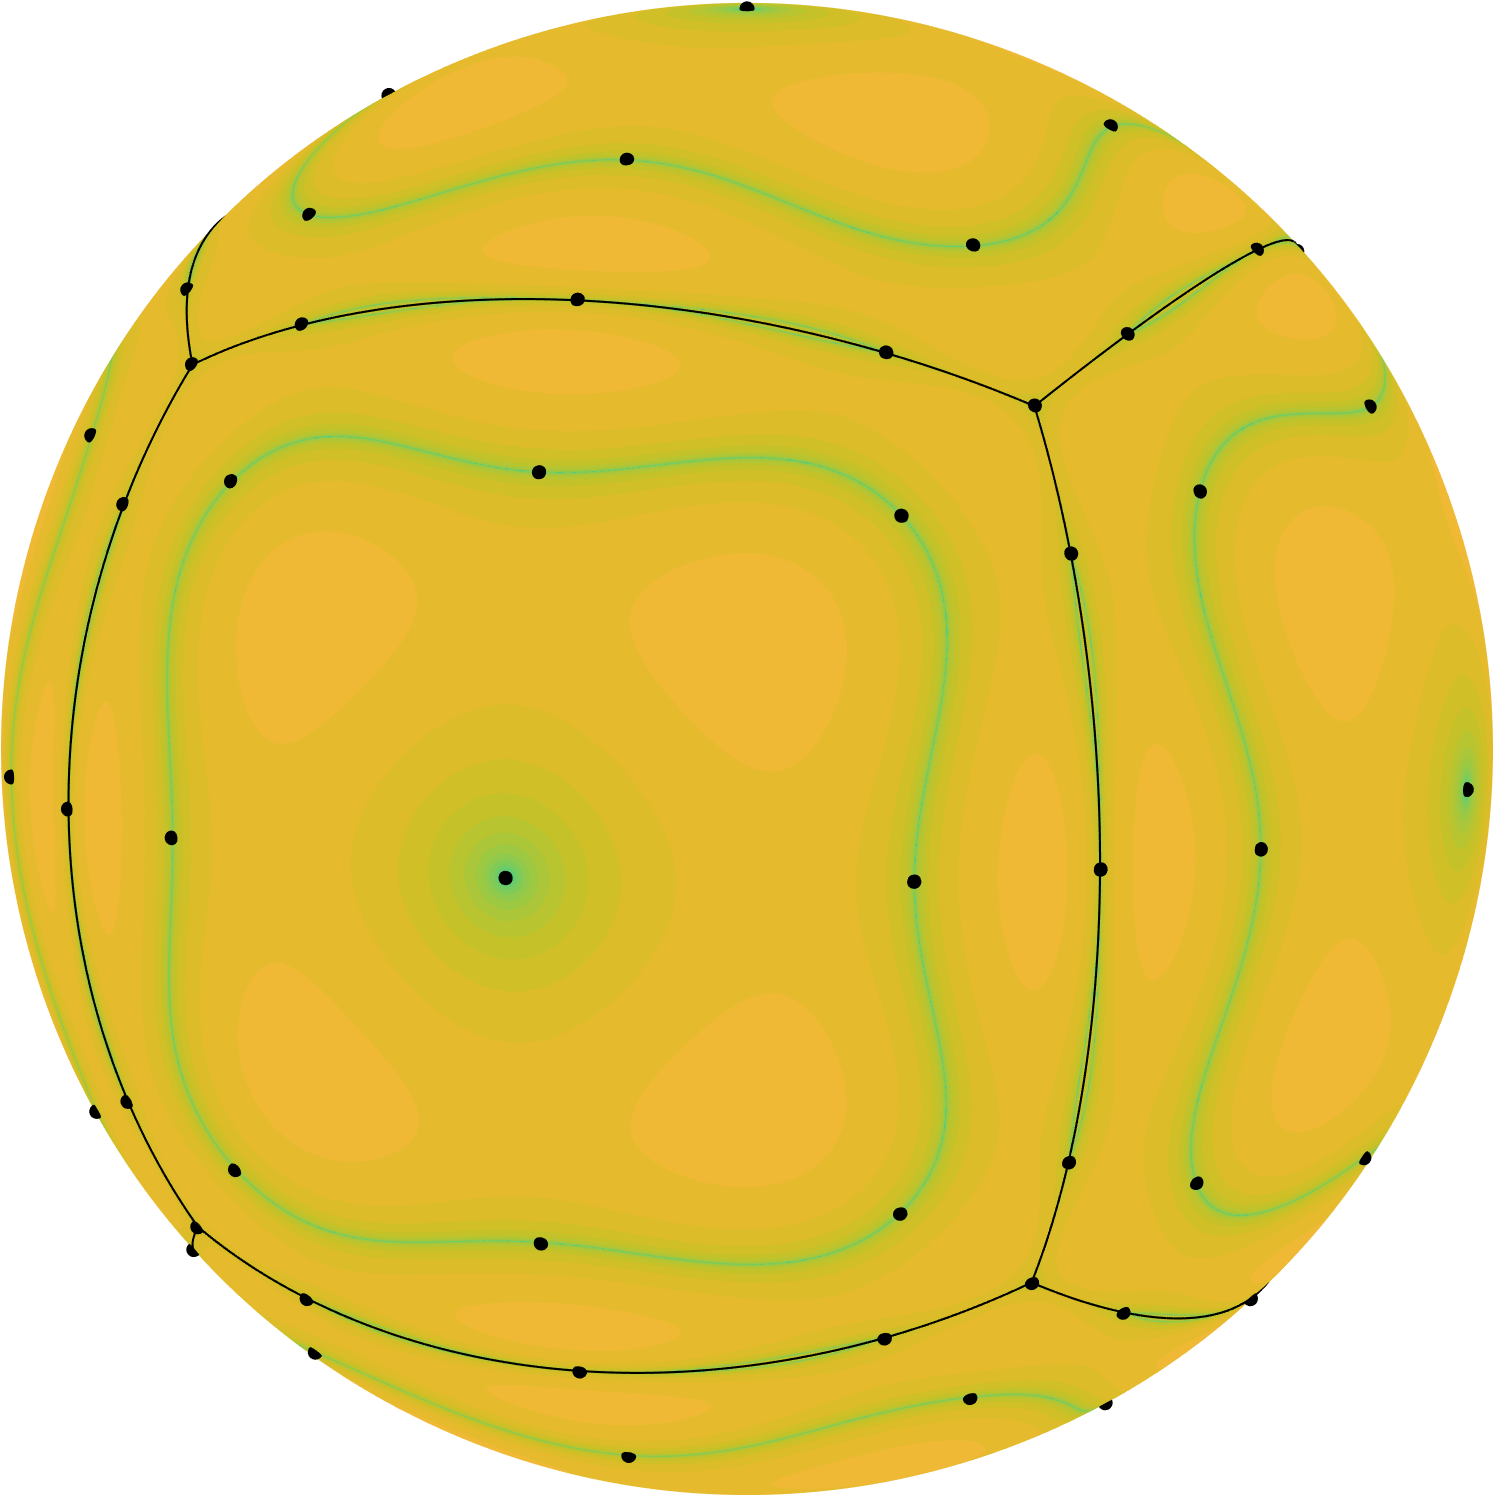
\includegraphics[width=\textwidth]{../../graphics/S1/SEM_p4}
		\caption{$p_\upxi=p_\upeta=p_\upzeta=4$}
	\end{subfigure}%
	\hspace*{0.01\textwidth}%
	\begin{subfigure}[t]{0.28\textwidth}
		\centering
		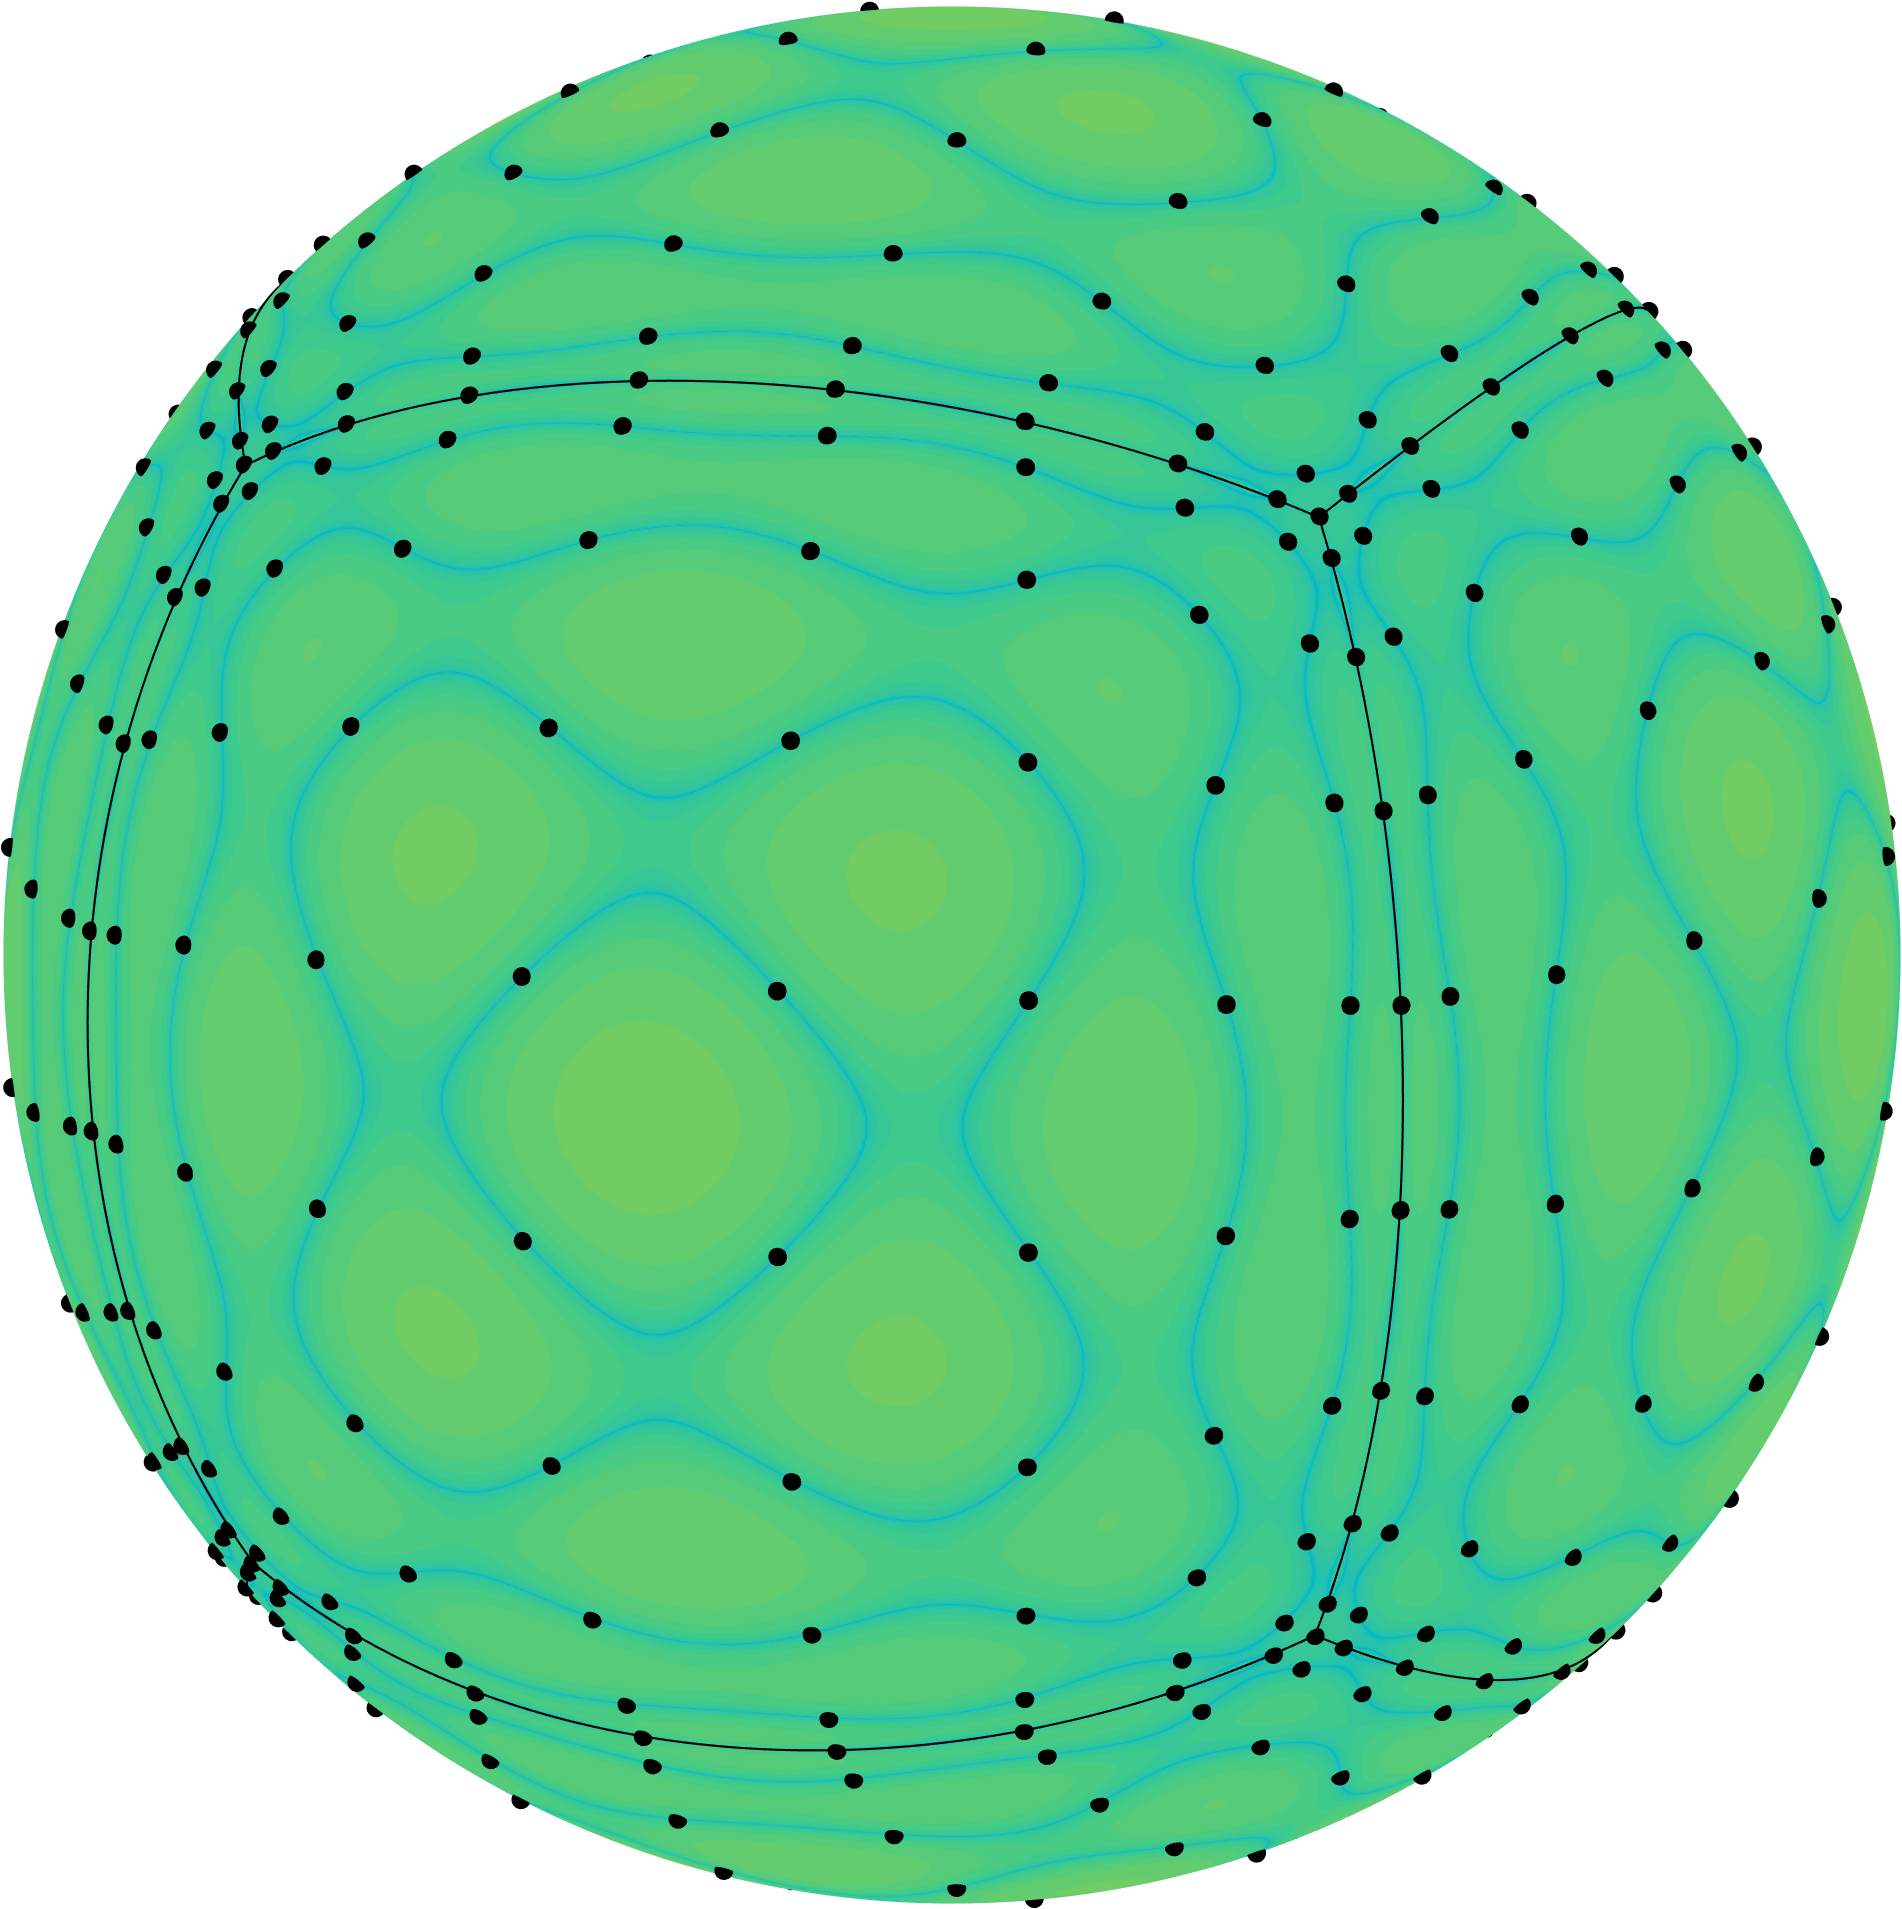
\includegraphics[width=\textwidth]{../../graphics/S1/SEM_p9}
		\caption{$p_\upxi=p_\upeta=p_\upzeta=9$}
	\end{subfigure}%
	\hspace*{0.01\textwidth}%
	\begin{subfigure}[t]{0.28\textwidth}
		\centering
		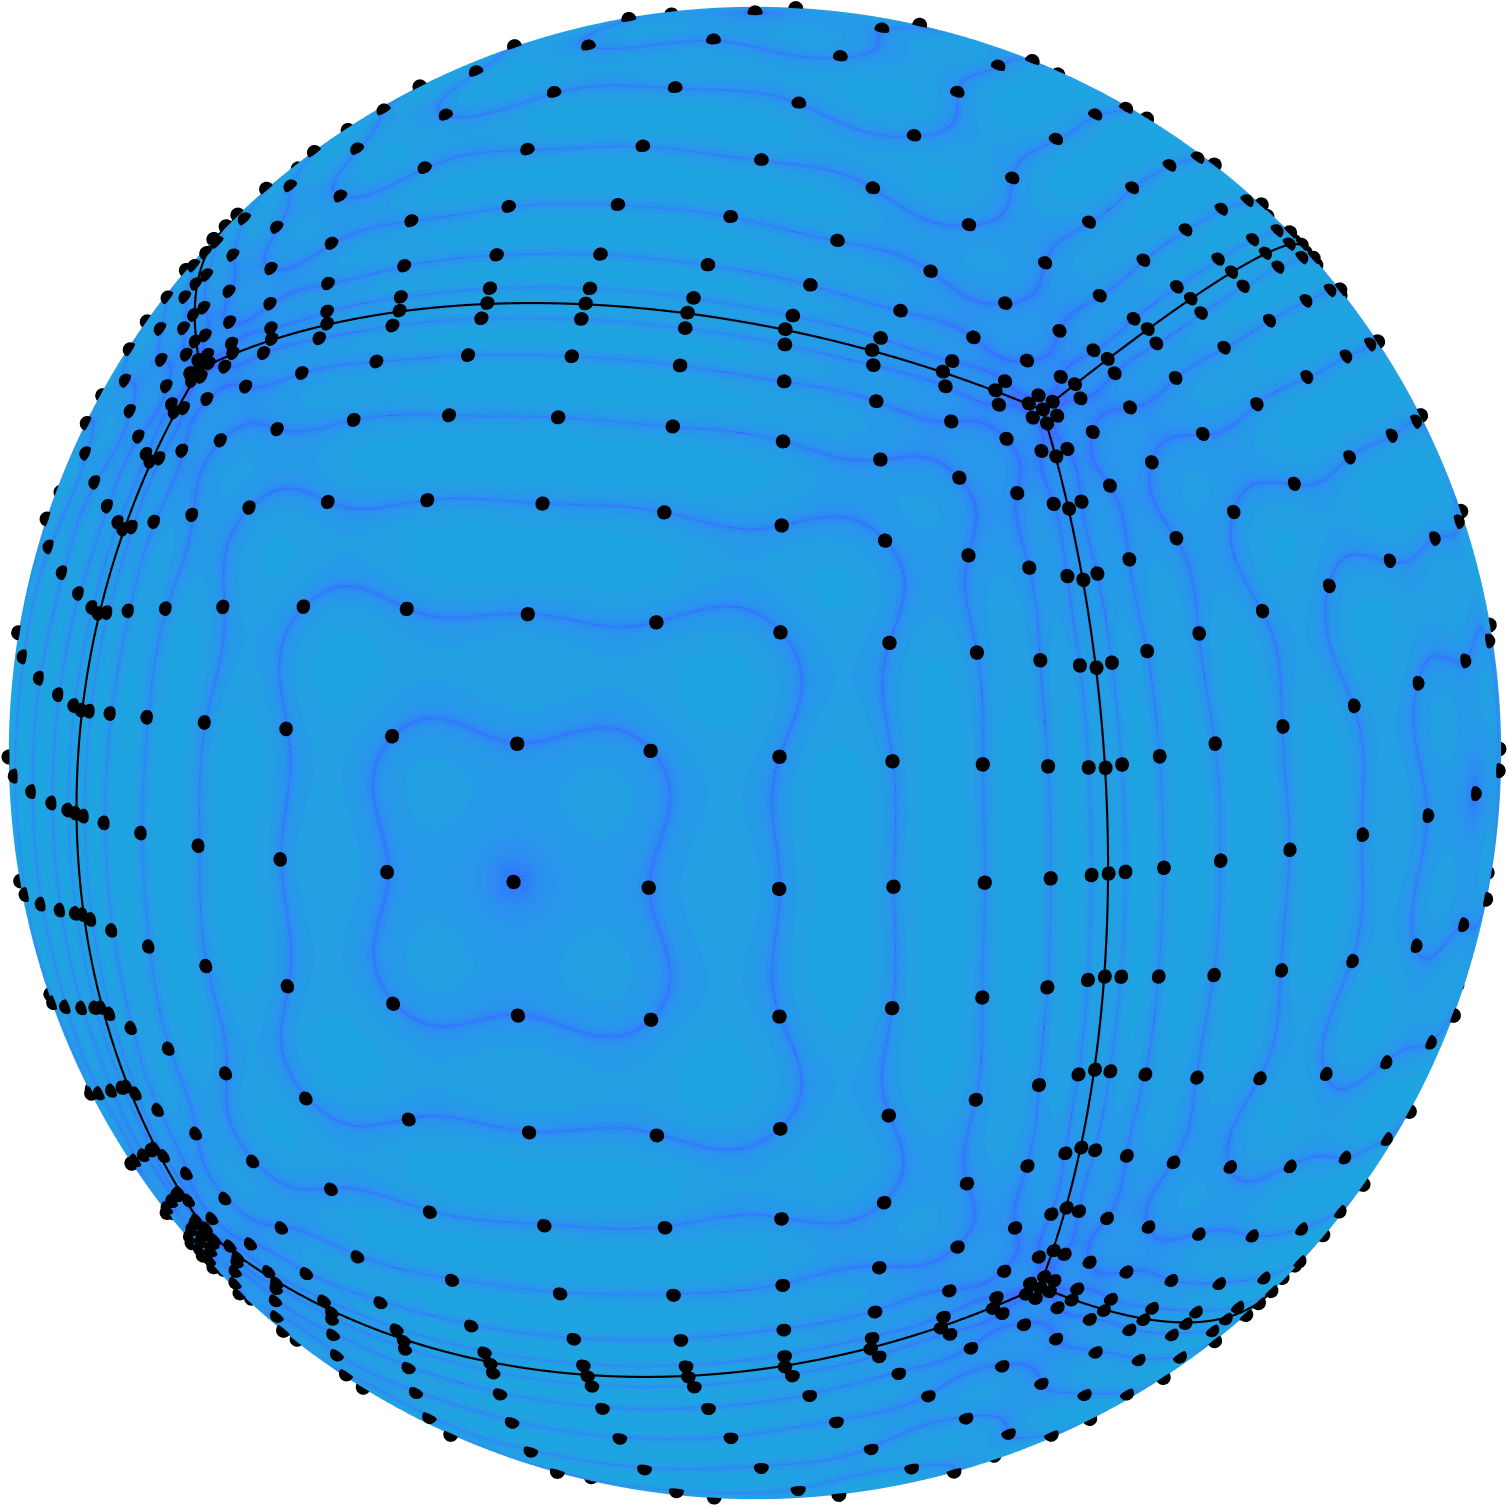
\includegraphics[width=\textwidth]{../../graphics/S1/SEM_p14}
		\caption{$p_\upxi=p_\upeta=p_\upzeta=14$}
	\end{subfigure}%
	\hspace*{0.01\textwidth}%
	\begin{subfigure}[t]{0.1\textwidth}
		\centering
		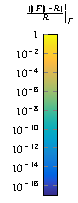
\includegraphics[width=\textwidth]{../../LaTeX/createFigures/TikzFigures/articleSEM_PhD/S1geometryApprox}
	\end{subfigure}
	\caption{Geometric error in the approximation of the sphere geometry using 6 patches. Machine epsilon precision is reached for polynomial degrees above 19. The approximation is based on the exact parametrization of a sphere using 6 NURBS patches.}
	\label{Fig5:spectralGeomteryApprox}
\end{figure}